\section{Motores de combustión Interna}

\begin{figure} \centering 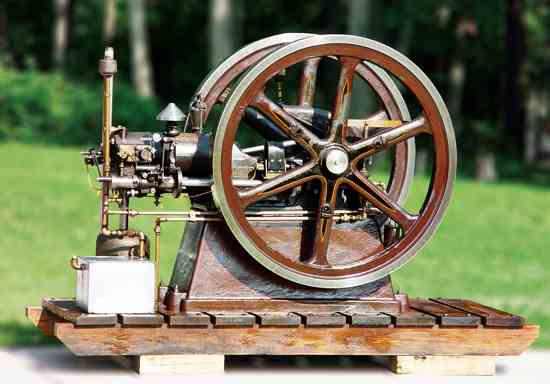
\includegraphics[width=.5\textwidth]{otto_1909.jpg}
    \caption{Motor 1909 5HP Otto Special Electric Lighting de Wayne
Grenning}\label{fig:otto1909} %
https://www.gasenginemagazine.com/gas-engines/1909-5-hp-otto-special-electric/
\end{figure}

Los motores de combustión interna dieron un impulso a la actividad humana desde
los años 1860, cuando su uso comercial comenzó a popularizarse.
%
La función de estos dispositivos es la de convertir energía potencial del fluido
de trabajo (una mezcla de aire-combustible) en trabajo mecánico por medio de un
proceso de combustión controlada dentro del cilindro o cámara de combustión.
%
Los primeros ejemplares comerciales eran voluminosos, costosos, altamente
ineficientes y de baja potencia, con valores de rendimiento cercano al 5\% y
potencias de hasta 6 HP.

Un paso importante hacia los motores actuales fue el desarrollo del ciclo Otto,
propuesto por Nicolaus A. Otto y Eugen Langen, cuyo primer prototipo se puso en
marcha en el año 1876.
%
Otto propuso un motor alternativo con cuatro carreras de pistón: admisión,
compresión, expansión y escape; este prototipo lograba la misma potencia con
mayor eficiencia que los motores de la época con menos de la mitad del peso y
volumen.
%
En la figura \ref{fig:otto1909} se ve un motor de ciclo Otto fabricado por
\emph{Otto Gas Engines Works} en el año 1909 en Filadelfia-EEUU, según la
revista \emph{Gas Engine
Magazine}\footnote{\url{https://www.gasenginemagazine.com/gas-engines/1909-5-hp-otto-special-electric/}}
\footnote{ \url{https://www.youtube.com/watch?v=LPSWfg0Y3Hs} } \footnote{
\url{https://www.youtube.com/watch?v=0d0WZ0H56_U} } este motor funcionaba
directamente acoplado a una bomba \emph{triplex} de agua, como parte de un
sistema de irrigación de un club de campo de Delaware.
%
Los motores han continuado su desarrollo desde entonces, mejorando materiales,
combustibles y procesos de manufactura entre otros aspectos.
%
En las últimas décadas se ha hecho foco en disminuir el consumo de combustible,
nivel de ruido, costo de manufactura, tamaño y las emisiones de gases de
contaminantes y de efecto invernadero como las de $CO_2$, $CO$ y $NO_x$, entre
otras.


El ciclo operativo de cuatro tiempos de Otto se puede expresar en términos de
carreras del pistón (\ref{fig:4tiempos}) en la que pueden identificar dos
posiciones de interés: punto muerto superior (PMS) y el punto muerto inferior
(PMI).
%
En el PMS se tiene el volumen mínimo atrapado en el cilindro y el pistón está al
final de la carrera, en el punto más alejado del eje del cigüeñal.
%
El PMI es el punto en el que se tiene el volumen máximo del cilindro y el pistón
está en el punto más cercano al eje del cigüeñal, como se ve en la
figura~\ref{fig:pms_pmi}.
%
Las carreras de pistón del ciclo Otto son:
%
\begin{description}
%
    \item [Carrera de admisión] El pistón se mueve desde el PMS hasta el PMI con
la válvula de admisión abierta y la de escape cerrada, esto hace que ingrese una
masa de aire o aire-combustible al cilindro.
%
    \item [Carrera de compresión] El pistón se mueve desde el PMI hacia el PMS
con la válvula de admisión y escape cerradas, esta reducción del volumen
comprime y calienta los gases en el interior del cilindro.
        %
        En una posición angular del ciclo denominada \emph{avance de encendido}
se enciende la mezcla y comienza la combustión.
%
    \item [Carrera de potencia o expansión] La combustión produce un gran
aumento de presión y temperatura en el cilindro, la carrera de expansión parte
del PMS hacia el PMI, aprovechando la expansión en volumen de los productos de
la combustión que producen trabajo sobre la cara del pistón.
%
    \item [Carrera de escape o barrido] Luego de la carrera de expansión,
próximo al PMI se abre la válvula de escape y el movimiento del pistón hacia el
PMS produce un barrido de los gases quemados, reiniciando el ciclo.
%
\end{description}

\begin{figure}
  \centering
  \begin{subfigure}{0.6\textwidth}
    \centering
    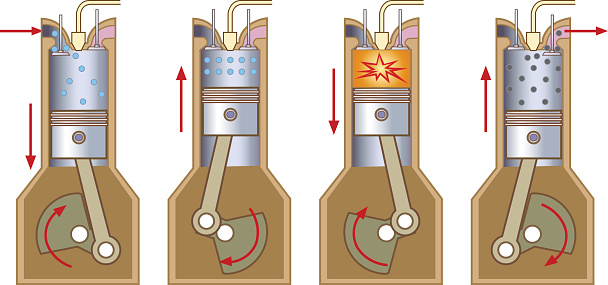
\includegraphics[width=\textwidth]{4stroke.jpg}
    \caption{Ciclo de cuatro tiempos}\label{fig:4tiempos} %
  \end{subfigure}%
  \begin{subfigure}{0.4\textwidth}
    \centering
    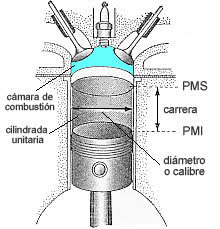
\includegraphics[width=\textwidth]{pms_pmi.jpg}
    \caption{PMS y PMI}\label{fig:pms_pmi}
  \end{subfigure}
  \caption{Ciclo de cuatro tiempos}
\end{figure}

% https://www.istockphoto.com/es/vector/motor-di%C3%A9sel-de-cuatro-tiempos-gm586705100-100702521

\subsection{Motores rotativos}
%
Los motores rotativos son una variable al diseño de los motores alternativos, su
compacidad, balanceo y mayores velocidades de giro los vuelven más atractivos en
aplicaciones en las cuales el volumen es restringido.
%
La mayor velocidad de giro permite alcanzar mayores potencias por lo que tiene
una menor relación peso/potencia que motores reciprocantes de potencia similar.
%
El diseño rotativo más conocido es el Wankel, cuyo primer prototipo funcional se
desarrolló cerca del año 1957.
%
Existen otros desarrollos de este tipo de motores como el motor
rotativo de pistón líquido, con un ciclo de combustión a volumen constante
denominado HECH\parencite{hehc_05} y el objeto de este traajo, el Motor Rotativo
de Combustión a Volumen Constante (MRCVC).

Si bien estos motores son una alternativa interesante a los motores
reciprocantes, la geometría y aspectos constructivos requiere introducir aceite
en la cámara de combustión para lubricar las partes móviles, además tienen una
mayor superficie de transferencia de calor causando una mayor pérdida de calor
en comparación con los motores reciprocantes.
%
En la actualidad, los requisitos de niveles de emisiones ambientales de ciertos
gases hacen estos motores inviables para el uso comercial, sin embargo la
compacidad del motor los vuelve atractivos en aplicaciones militares como por
ejemplo para vehículos aéreos no tripulados.

%%%%%%%%%%%%%%%%%%%%%%%%%%%%%%%%%%%%%%%%%%%%%%%%%%%%%%%%%%%%%%%%%%%%%%%%%%%%%%%


\subsection{Parámetros Operativos e Indicadores de rendimiento}
%
Para poder comparar entre diferentes diseños de motores se deben conocer algunos
parámetros operativos e indicadores de rendimiento, algunas de las
características más importantes de un motor son:
%
\begin{enumerate}
        %
    \item Potencia y torque
        %
    \item Rango de velocidades de operación
        %
    \item Consumo y costo de combustible
        %
    \item Costo inicial, de operación y de mantenimiento
        %
    \item Confiabilidad
        %
    \item Niveles de ruido y emisiones contaminantes
        %
\end{enumerate}

Estas características se pueden expresar de manera más genérica en función de la
potencia, geometría u otros aspectos de un motor para obtener valores que se
pueden comparar directamente entre motores.
%
Por ejemplo, al cociente entre el trabajao entregado por ciclo y la cilindrada
de un motor se lo conoce como presión media efectiva o \emph{mep}, por sus
siglas en inglés.
%
Algunos parámetros operativos e indicadores se describen en los párrafos
siguientes.

%%%%%%%%%%%%%%%%%%%%%%%%%%%%%%%%%%%%%%%%%%%%%%%%%%%%%%%%%%%%%%%%%%%%%%%%%%%%%%%

\subsubsection{Volumen Desplazado}
%
El volumen desplazado se define como la diferencia entre el volumen máximo y
mínimo que ocupa la cámara de combustión.

\begin{equation}\label{eq:vol_desp} V_d = V_{max}-V_{min}
\end{equation}

% La geometría de la càmara de combustión del MRCVC está definida por leyeEn el
% MRCVC la geomeria de la cámara de combustión es m'0

%%%%%%%%%%%%%%%%%%%%%%%%%%%%%%%%%%%%%%%%%%%%%%%%%%%%%%%%%%%%%%%%%%%%%%%%%%%%%%%

\subsubsection{Relación de compresión}

Se define como el cociente ente el volumen máximo y el volumen mínimo del ciclo,
es uno de los parámetros más importantes de un motor ya que afecta la presión
máxima que se puede obtener en la cámara de combustión, \emph{performance},
potencia entregada, esfuerzos mecánicos y rendimiento del motor.

\begin{equation}\label{eq:rel_comp} r_c = \frac{V_{max}}{V_{min}} = \frac{V_d+V_c}{V_c}
\end{equation}

%%%%%%%%%%%%%%%%%%%%%%%%%%%%%%%%%%%%%%%%%%%%%%%%%%%%%%%%%%%%%%%%%%%%%%%%%%%%%%%

% \subsubsection{Troque y potencia al freno} % NOTA: Hace flata?

%%%%%%%%%%%%%%%%%%%%%%%%%%%%%%%%%%%%%%%%%%%%%%%%%%%%%%%%%%%%%%%%%%%%%%%%%%%%%%%

\subsubsection{Trabajo indicado por ciclo}
%
El trabajo entregado por el cilindro al cigüeñal por cada ciclo de operación
se denomina trabajo indicado por ciclo y se obtiene al integrar la presión
en función del volumen, es el área encerrada en un diagrama de P-V del motor.

\begin{equation}\label{eq:w_indicado} W_{c,i} = \oint P dV
\end{equation}

Se debe diferenciar entre trabajo bruto y trabajo neto, en el último se tiene en
cuenta el trabajo de bombeo que resulta de la diferencia del trabajo realizado
durante las carreras de admisión y escape, por lo que este indicador se puede
diferenciar en:
%
\begin{description}
  \item [Trabajo bruto indicado por ciclo] $W_{c,ig}$, mide el trabajo realizado
por el motor en las carreras de compresión y expansión.
  \item [Trabajo neto indicado por ciclo] $W_{c,in}$, mide el trabajo realizado
por el motor considerando las 4 carreras del ciclo.
  \item [Trabajo de bombeo] Es la diferencia entre el trabajo bruto y neto, mide
el trabajo realizado durante los procesos de admisión y escape.
  \item [Trabajo de fricción] Es el trabajo consumido por el rozamiento entre
partes móviles del motor.
\end{description}

% TODO, 15/07 agregar una figura con el área bajo la curva del diagrama P-V y si
% puedo indicar los trbajos de bombeo, bruto y neto, mejor

%%%%%%%%%%%%%%%%%%%%%%%%%%%%%%%%%%%%%%%%%%%%%%%%%%%%%%%%%%%%%%%%%%%%%%%%%%%%%%%

% \subsubsection{Rendimiento Mecánico}

%%%%%%%%%%%%%%%%%%%%%%%%%%%%%%%%%%%%%%%%%%%%%%%%%%%%%%%%%%%%%%%%%%%%%%%%%%%%%%%

\subsubsection{Consumo especifico de combustible y rendimiento de conversión de
combustible}
%
El consumo especifico de combustible \emph{sfc}, se define como el cociente
entre el caudal másico de combustible ($\dot{m_f}$) consumido por unidad de
potencia $P$ entregada por el motor.

\begin{equation}\label{eq:sfc} sfc = \frac{\dot{m_f}}{P}
\end{equation}

Mide la eficiencia con la que el motor utiliza el combustible para una condición
de operación dada, en motores de encendido por chispa se tienen valores típicos
para de alrededor de $65\mu g/J$.

Una versión similar de este indicador adimensionalizado en relación a la energía
suministrada por el combustible, es el \emph{rendimiento de conversión de
combustible} $\eta_f$, que se relaciona al \emph{sfc} por medio del poder
calórico del combustible, $Q_{HV}$.

\begin{equation}\label{eq:eta_f} \eta_f = \frac{1}{sfc \cdot Q_{HV}}
\end{equation}

El valor de $Q_{HV}$ es una propiedad del combustible que se determina en un
ensayo de laboratorio, valores típicos para los combustible comerciales basados
en hidrocarburos son 42 a 44 $MJ/kg$

%%%%%%%%%%%%%%%%%%%%%%%%%%%%%%%%%%%%%%%%%%%%%%%%%%%%%%%%%%%%%%%%%%%%%%%%%%%%%%%

\subsection{Presión Media Efectiva}
%
La presión media efectiva o $mep$ por sus siglas en inglés es un indicador cuya
variación es similar a la curva de torque pero adimensionalizada por el tamaño
de cada motor.
%
El trabajo realizado por ciclo se puede calcular como
$W_c = \frac{P \cdot n_r}{N}$, donde $n_R$ es el número de revoluciones del
cigüeñal por cada carrera de expansión por cilindro.
%
Para motores de cuatro tiempos $n_R=2$ y $n_R=1$ para motores de dos tiempos,
con esto la presión media efectiva se define como:

\begin{equation}\label{eq:mep} mep = \frac{W_{c}}{V_d} = \frac{P \cdot n_R}{V_d \cdot N}
\end{equation}

Se puede diferenciar entre presión media efectiva indicada (\emph{imep}), al
freno (\emph{bmep}) y de fricción (\emph{fmep}), utilizando el valor de potencia
correspondiente en la ecuación \ref{eq:mep}.
%
El valor de \emph{mep} (al igual que el torque) de un motor varía con la
velocidad de operación, siguiendo de cerca la curva de rendimiento volumétrico
como se puede ver en la figura~\ref{fig:bmep_tipica}.

En la actualidad, valores típicos de \emph{bmep} de motores SI naturalmente
aspirados rondan los 1050 kPa a 1250 kPa para la velocidad a la que se alcanza
el torque máximo.

\begin{figure} \centering
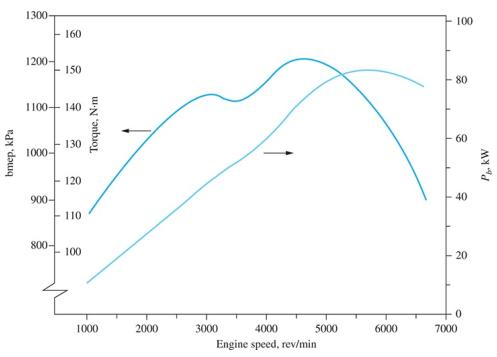
\includegraphics[width=0.7\textwidth]{curva_bmep_tipica.jpg}
    \caption{\emph{bmep}, torque y potencia vs velocidad de
operación\parencite{heywood}.}
    \label{fig:bmep_tipica}
\end{figure}

%%%%%%%%%%%%%%%%%%%%%%%%%%%%%%%%%%%%%%%%%%%%%%%%%%%%%%%%%%%%%%%%%%%%%%%%%%%%%%%

\subsection{Rendimiento Volumétrico}
%
El rendimiento volumétrico mide la eficiencia del sistema de admisión y se
define como el cociente entre el caudal másico de aire que ingresa al sistema de
admisión y la velocidad con la que este volumen es desplazado por el pistón.
%
En otras palabras, este indicador mide la eficiencia con la que el motor bombea
aire.

\begin{equation}\label{eq:eta_v} \eta_v = \frac{2\dot{m_a}}{\rho_{a,i}V_d N} = \frac{m_a}{\rho_{a,i}V_d}
\end{equation}

Para motores naturalmente aspirados la densidad del aire de admisión
$\rho_{a,i}$ se toma comúnmente como la densidad atmosférica por lo que $\eta_v$
mide el rendimiento de todo el sistema de admisión.

El valor de rendimiento volumétrico máximo para motores naturalmente aspirados
ronda el 90\%.
%
Su valor se ve afectado por varios fenómenos dentro de los cuales los más
importantes son:

\begin{description}
        %
    \item [Efectos cuasiestáticos] Combustible, relación aire/combustible,
vaporización del combustible en el conducto de admisión, temperatura del aire de
admisión, relación entre presión de admisión y escape, relación de compresión,
etc.
  \item [Pérdidas de carga por fricción viscosa] Las pérdidas viscosas aumentan
con la velocidad de flujo y aumentan a medida que aumenta la velocidad de giro
del motor.
        %
  \item [Pérdidas de carga localizada] Filtros, puertos, válvulas generan
pérdidas localizadas, caídas de presión.
        %
  \item [Transferencia de calor en sistema de admisión] La mezcla se calienta
por transferencia de calor y esto disminuye la densidad de la misma, reduciendo
la masa disponible para la combustión.
        %
  \item [Reglaje de las válvulas/puertos] El punto de apertura y cierre de los
puertos (reglaje) es clave para el funcionamiento del motor, dependiendo del
reglaje que se elija, se puede favorecer el flujo a determinada velocidad de
operación.
        %
    \item [Flujo bloqueado en puertos de admisión y escape] En las zonas de
menor área de pasaje la velocidad del fluido puede aumentar hasta alcanzar la
velocidad del sonido, esto se conoce como bloqueo y limita el caudal másico que
puede ingresar a la cámara de combustión.
        %
%     \item [Transferencia de calor en el cilindro] La cámara de combustión se %
% encuentra a mayor temperatura que la mezcla que ingresa, esto produce un aumento
% del volumen específico reduciendo la cantidad que puede ingresar.
        %
    \item [Sintonía del puerto de admisión y escape] El diseño de los puertos de
admisión y escape puede favorecer el funcionamiento de los mismos a determinada
velocidad de operación, esto se logra aprovechando las ondas de presión que se
producen por la apertura y cierre de las válvulas.
        %
  \item [Sobrecarga] Por medio de un compresor o turbocompresor se puede
aumentar presión en el sistema de admisión forzando más aire a la cámara de
combustión.
        %
    \item [Efecto RAM] A grandes velocidades de flujo la inercia del gas produce
un aumento de presión al momento del cierre del puerto de admisión y esto
permite un mayor ingreso de masa fresca al cilindro.
        %
\end{description}

La curva de rendimiento volumétrico es muy similar a la curva de torque o de
presión media efectiva, la cantidad de aire que ingresa al motor está
directamente relacionada con el trabajo que puede realizar por ciclo de
operación.
%
Este indicador es central en la evaluación del desempeño de los sistemas de
intercambio de gases y por este motivo es el principal indicador utilizado en
este trabajo.
%
En este trabajo se busco que la curva de rendimiento volumétrico de los motores
simulados tenga un máximo para velocidades mayores a 6000 RPM para de aprovechar
el balanceo mecánico del motor que permite funcionar y seguir entregando
potencia a altas RPM además, la curva debe ser preferentemente suave para todo
el régimen de funcionamiento del motor.

Estos y otros efectos se describen en detalle en la
literatura~\parencite{heywood}, para este trabajo se realizaron las siguientes
consideraciones:

\begin{enumerate}
        %
    \item El combustible utilizado es isooctano, la mezcla aire-combustible es
estequeométrica ($\phi=1$).
        %
    \item El sistema de intercambio de gases del MRCVC se compone de un conducto
y puerto admisión, conducto y puerto de escape.
        %
        ICESym tiene en cuenta pérdidas por fricción viscosa en los conductos,
los puertos generan pérdidas localizadas.
        %
    \item Los conductos se asumen como elementos rectos de un largo finito y
diámetro constante, cuya fuente y sumidero es la atmósfera a $101330 Pa$ y
$25^{\circ}C$.
        %
    \item La temperatura de la pared de la cámara de combustión se asume en
450K.
        %
    \item El motor es naturalmente aspirado.
        %
\end{enumerate}

\subsection{Fracción de gases residuales}
%
La fracción de gases residuales $x_r$ mide la cantidad de gases quemados que hay
en el cilindro al inicio de la carrera de admisión.
%
La masa residual en la cámara de combustión es producto de dos efectos, en
primer lugar al momento del cierre de la válvula de escape quedan gases
residuales de la combustión atrapados en el cilindro y en segundo lugar puede
existir un reflujo desde el puerto de escape hacia la cámara de combustión por
haber solape de válvulas.

La fracción de gases residuales afecta el rendimiento volumétrico, trabajo
obtenido, eficiencia y emisiones.

\begin{equation}
    x_{r} = \frac{m_{r}}{m}
\end{equation}

En el MRCVC existe además solape de cámara, este es un fenómeno en el que una
cámara en proceso de admitir gases frescos se ve afectada por la apertura del
puerto de admisión a la cámara siguiente, que se encuentra a mayor presión y
temperatura por estar culminando el proceso de escape y comenzando el de
admisión, esto aumenta la cantidad de gases residuales.
%
Una menor fracción de gases residuales tiene dos efectos beneficiosos, en
primer lugar estos gases ocupan volumen en la cámara de combustión, además
porque su elevada temperatura (en relación a la masa fresca) calienta el gas que
ingresa al cilindro desde el puerto de admisión, aumentando el volumen
específico y reduciendo el rendimiento volumétrico.



\subsection{Coeficiente de descarga}
%
La pérdida de carga localizada en los puertos de admisión y escape se puede
medir con el coeficiente de descarga $C_{D}$, este indicador mide la eficiencia
del escurrimiento y se obtiene experimentalmente o con simulaciones
computacionales.
%
El valor de $C_{D}$ varía con la geometría y condiciones de operación del
puerto, siendo $C_{D}=1$ el caso ideal sin pérdida de carga localizada.

El caudal másico ($\dot{m}$) que circula por los puertos se calcula a partir de
las ecuaciones de flujo compresible a través de una restricción, para el caso en
que el flujo no esté bloqueado la ecuación de $\dot{m}$ es
la~\ref{eq:m_no_bloqueado} y en caso de que se cumpla la
desigualdad~\ref{eq:cond_bloqueo} el flujo está bloqueado y se utiliza la
ecuación~\ref{eq:m_bloqueado}.
%

\begin{equation}\label{eq:m_no_bloqueado}
  \dot{m} = \frac{C_D A_R p_0}{\sqrt{R T_0}} {\left(\frac{p_T}{p_0} \right)}^{1/\gamma} {\left( \frac{2\gamma}{\gamma-1} \left[1- {(\frac{p_T}{p_0})}^{{\gamma-1}/\gamma} \right] \right)}^{1/2}
\end{equation}

\begin{equation}\label{eq:cond_bloqueo}
  \frac{p_T}{p_0} \le {[\frac{2}{\gamma+1}]}^{\gamma/(\gamma - 1)}
\end{equation}

\begin{equation}\label{eq:m_bloqueado}
  \dot{m}=  \frac {C_D A_R p_0} {{(R T_0)}^{1/2}} \gamma^{1/2} {\left( \frac{2\gamma}{\gamma+1} \right)}^{(\gamma+1)/(2(\gamma-1))}
\end{equation}

Dónde:

\begin{itemize}
    \item $p_0$, es la presión de estancamiento antes de la restricción.
    \item $T_0$, es la temperatura de estancamiento antes de la restricción.
    \item $p_T$, es la presión estática justo después de la restricción.
    \item $A_R$, es el área de pasaje de flujo o de referencia.
    \item $\dot{m}$, es el caudal másico.


  \item $\gamma$, es el cociente de capacidades térmicas del gas.
\end{itemize}

Las presiones y temperaturas involucradas en el cálculo de $\dot{m}$ se pueden
medir u obtener de una simulación computacional del ciclo del motor.
%
La elección del área de referencia utilizada para el cálculo es arbitraria, sin
embargo se suele utilizar el área de cortina, que se calcula como con el
producto del diámetro $D_{v}$ y alzada de válvula $l_{v}$.

\begin{equation} \label{eq:area_cortina} A_R = A_C = \pi D_v l_v
\end{equation}

\begin{figure} \centering
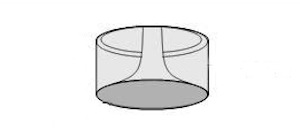
\includegraphics[width=0.5\textwidth]{valve_curtain.jpg}
  \caption{Área de cortina}\label{fig:area_cortina}
\end{figure}


%%%%%%%%%%%%%%%%%%%%%%%%%%%%%%%%%%%%%%%%%%%%%%%%%%%%%%%%%%%%%%%%%%%%%%%%%%%%%%%
\subsection{Sincronización del sistema de admisión}
%
En motores naturalmente aspirados, al momento de abrir la válvula o puerto de
admisión, los gases residuales en la cámara se encuentran a una presión mayor
que la masa fresca en el puerto de admisión, esta diferencia de presión produce
una onda de depresión que viaja desde la cámara de combustión hacia el extremo
opuesto del conducto de admisión.
%
Cuando esta onda de presión llega al plenum de admisión, se refleja como una
onda de sobrepresíon que toma un tiempo $t$ en alcanzar nuevamente el puerto, si
el tiempo que toma la onda en reflejarse es tal que alcanza la válvula justo
antes del cierre de la misma el sistema está sintonizado.
%
Esta sopbrepresión permite que ingrese una mayor cantidad de masa fresca a la
cámara de combustión, aumentando la cantidad de trabajo que se puede realizar.

En la figura~\ref{fig:sintonia1} se muestra el diagrama de presión vs ángulo de
cigüeñal para 1200 y 4800 RPM, en donde se indican los períodos en los que se
encuentran abiertos las válvulas de admisión (IO) y de escape (EO).
%
% En la figura xxx se muestra un diagrama de presión vs ángulo de cigüeñal de una de las simulaciones realizadas del MRCVC y en la figura xxx se representa la curva de rendimiento volumétrico del motor. Se ve que para a 6000 RPM se tiene $\eta_{v,\max}$ y observando las curvas de presión del puerto de admisión y escape se nota una sintonía en el puerto de admisión y otra en el puerto de escape. Este motor tiene un rendimiento volumétrico un 20% menor para 1500 RPM, observando las curvas de presión en l
%
Los valores $p_1$, $p_2$ y $p_3$ hacen referencia diferentes longitudes de los
conductos de admisión y escape.
%
Se puede ver que para $p_1$ a 4800 RPM hay un claro pico de presión justo al
cierre del puerto de admisión, con esto el puerto está sintonizado para esta
velocidad.

\begin{figure} \centering
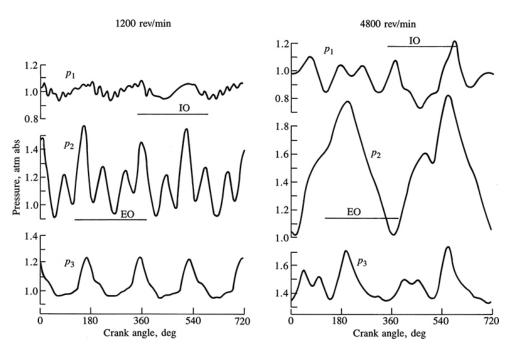
\includegraphics[width=0.7\textwidth]{sintonia_heywood.jpg}
    \caption{(cambiar por una del mrcvc) Diagrama de presión vs ángulo de
cigüeñal}\label{fig:sintonia1}
\end{figure}

Debido a que la onda de presión debe viajar dos veces longitud del conducto de
admisión desde el momento que abre el puerto de admisión, para sincronizar el
sistema de admisión a bajas velocidades, se requieren longitudes mayores lo que
hace más grande el sistema de admisión.
%
La sincronía a mayores velocidades de admisión es preferida, porque usualmente
se tiene el máximo de torque y de potencia a mayores RPM, además reduce la
necesidad de conductos más largos.
%
En motores multi-cilíndricos se utiliza un plenum de admisión, este dispositivo
proporciona un volumen grande de aire que sirve el propósito de cámara de
resonancia.
%
Se puede ajustar la resonancia de modo que las oscilaciones de presión internas
produzcan ondas de sobre presión que alcancen cada puerto en el momento preciso
en el que se aproxima el cierre del mismo.

%%%%%%%%%%%%%%%%%%%%%%%%%%%%%%%%%%%%%%%%%%%%%%%%%%%%%%%%%%%%%%%%%%%%%%%%%%%%%%%

\subsection{Sincronización del sistema de escape}

De forma análoga al puerto de admisión, al momento de la apertura del puerto o
válvula de escape los gases residuales de la combustión se encuentran a  mayor
presión que el gas en el conducto, esto crea una onda de sobrepresión que viaja
por el escape hasta alcanzar el final del mismo o un área de gran volumen, como
el catalizador o el silenciador.
%
Desde esta zona se refleja como una onda de depresión, que en caso de alcanzar
el puerto en los instantes previos al cierre del mismo, ayuda a evacuar una
mayor cantidad de gas, disminuyendo la fracción de gases residuales.

En la figura \ref{fig:sintonia1} se ve que para el escape en $p_2$ se tiene una
depresión justo al cierre del puerto, este sistema está sintonizado para 4800
RPM, es notorio el contrate con el mismo puerto a 1200 RPM, en donde se ve un
pico de presión cerca del cierre del puerto.

%%%%%%%%%%%%%%%%%%%%%%%%%%%%%%%%%%%%%%%%%%%%%%%%%%%%%%%%%%%%%%%%%%%%%%%%%%%%%%%

\subsection{Combustión}
%
La combustión es un proceso en el que se libera la energía química del
combustible, la geometría de un motor de combustión interna permite aprovechar
el aumento de presión y temperatura para convertir energía química en trabajo
mecánico.
%
Los modelos ideales de ciclos operativos se pueden clasificar según el proceso
de combustión en:
%
\begin{enumerate}
        %
    \item Volumen constante, fig.~\ref{fig:comb_vcte}.
        %
    \item Presión constante, fig.~\ref{fig:comb_vcte}.
        %
    \item Presión limitada (parte a volumen constante y parte a presión
constante), fig.~\ref{fig:comb_plim}.
        %
\end{enumerate}

En un motor de encendido por chispa se tiene una mezcla de aire-combustible en
la cámara de combustión, dependiendo del tipo de motor la mezcla se puede formar
en el conducto de admisión, inyectando combustible en algún punto del sistema ó
se puede producir la mezcla en la cámara por la inyección directa de
combustible.
%
En un motor de encendido por compresión, la mezcla combustible se forma en la
cámara de combustión, la inyección de combustible se realiza directamente en la
cámara, cerca del PMS al final de la carrera de compresión.
%
Las condiciones de presión y temperatura dentro de la cámara producen el
auto-encendido de la mezcla y el inicio del proceso de combustión.

\begin{figure}[ht]
  \centering
  \begin{subfigure}{0.33\textwidth}
    \centering
    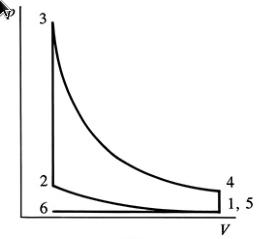
\includegraphics[width=\textwidth]{combustion_vol_cte.jpg}
    \caption{Volumen Constante}\label{fig:comb_vcte}
  \end{subfigure}%
  \begin{subfigure}{0.33\textwidth}
    \centering
    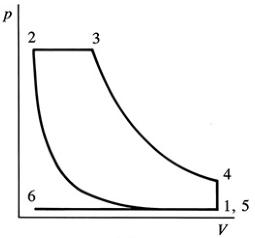
\includegraphics[width=\textwidth]{combustion_presion_cte.jpg}
    \caption{Presión Constante}\label{fig:comb_pcte}
  \end{subfigure}%
  \begin{subfigure}{0.4\textwidth}
    \centering
    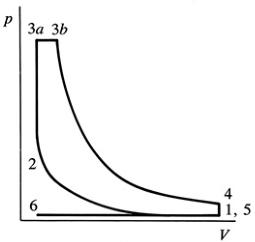
\includegraphics[width=\textwidth]{combustion_presion_limitada.jpg}
    \caption{Presión Limitada}\label{fig:comb_plim}
  \end{subfigure}
  \caption{Diagramas P-V para ciclos ideales\parencite{heywood}}\label{fig:ciclos_ideales}
\end{figure}

El MRCVC es un motor de combustión interna encendido por chispa en el que,
gracias al a geometría del mismo gran parte de la combustión ocurre a volumen
constante, esto se puede apreciar en la apreciar en la
figura~\ref{fig:mrcvc_vol_cte}, en la cual se gráfica la variación volumen en
función del ángulo del cigüeñal.
%
En este trabajo no se estudia el proceso de combustión del MRCVC, sin embargo se
describe el motivo por el que la combustión a volumen constante es una
característica atractiva de este motor.
%
% es más eficiente que la combustión a presión constante.

En \parencite{heywood} se hace un análisis de los modelos operativos de gas
ideal, en los cuales se asume que % El mayor rendimiento de la combustión a
volumen constante se puede ver % analizando los modelos ideales de ciclos
operativos \parencite{heywood}, el fluido de trabajo es gas ideal, con $C_v$ y
$C_p$ constantes.
%
Se pueden analizar los 3 casos de combustión: volumen constante, presión
constante o presión limitada, obteniendo expresiones para el rendimiento de
conversión de combustible~\ref{eq:rendimiento_p_lim} y de $imep$ en función de
la presión mínima del ciclo $p_1$~\ref{eq:imep_p1} y máxima
$p_3$~\ref{eq:imep_p3}.
%
Tanto la combustión a volumen constante como el caso a presión constante son
casos extremos de la combustión a presión limitada, por lo que se puede utilizar
el rendimiento de conversión de combustible para el ciclo de presión limitada es
para comparar entre ambos.

\begin{align}
    \label{eq:rendimiento_p_lim}
    %
    \eta_{f,i} &= 1 - \frac{1}{r_c^{\gamma - 1}} \left[ \frac{\alpha \beta^\gamma-1}{\alpha \gamma (\beta-1)+\alpha-1} \right]\\ \alpha &= \frac{P_3}{P_2}\\ \beta &= \frac{V_{3b}}{V_{3a}}
    %
\end{align}

\begin{equation}
    \label{eq:imep_p1} \frac{imep}{p_1} = \frac{Q^*}{c_v T_1 (\gamma-1)} \left( \frac{r_c}{r_c-1} \right) \eta_{f,i}
    %
\end{equation}

\begin{equation}
    \label{eq:imep_p3} \frac{imep}{p_3} = \frac{1}{\alpha r_c^\gamma} \left( \frac{Q^*}{c_v T_1} \right) \left(\frac{1}{\gamma-1} \right) \left( \frac{r_c}{r_c-1} \right) \eta_{f,i}
    %
\end{equation}

En el caso en que  $\alpha=1 \rightarrow P_3=P_2$ y se tiene el ciclo de
combustión a presión constante, en el caso en que
$\beta=1 \rightarrow V_{3a}=V_{3b}$ y se tiene el ciclo de combustión a volumen
constante, como se ve en la figura \ref{fig:ciclos_ideales}.

Graficando la ecuación \ref{eq:rendimiento_p_lim} en función de la relación de
compresión $r_c$ (figura \ref{fig:rendimientos}), para distintos valores se ve
que a igual relación de compresión, el ciclo a volumen constante presenta mayor
rendimiento de conversión de combustible.

Del mismo modo, graficando la relación entre la presión media efectiva indicada
y la presión máxima del ciclo, $imep/p_3$, se ve que a igual relación de
compresión el ciclo de combustión a presión constante presenta mayores valores
de $imep$ en relación a la presión máxima, esto tiene que ver con las altas
presión alcanzadas en el ciclo ideal de combustión a volumen constante.
%
La presión máxima que se puede alcanzar en el ciclo real tiene limitaciones
relacionadas a mayores pérdidas de masa (y presión) a través de sellos y la
resistencia mecánica de los componentes del motor además, mayores presiones
están asociadas con mayores temperaturas en la cámara de combustión.

\begin{figure} \centering
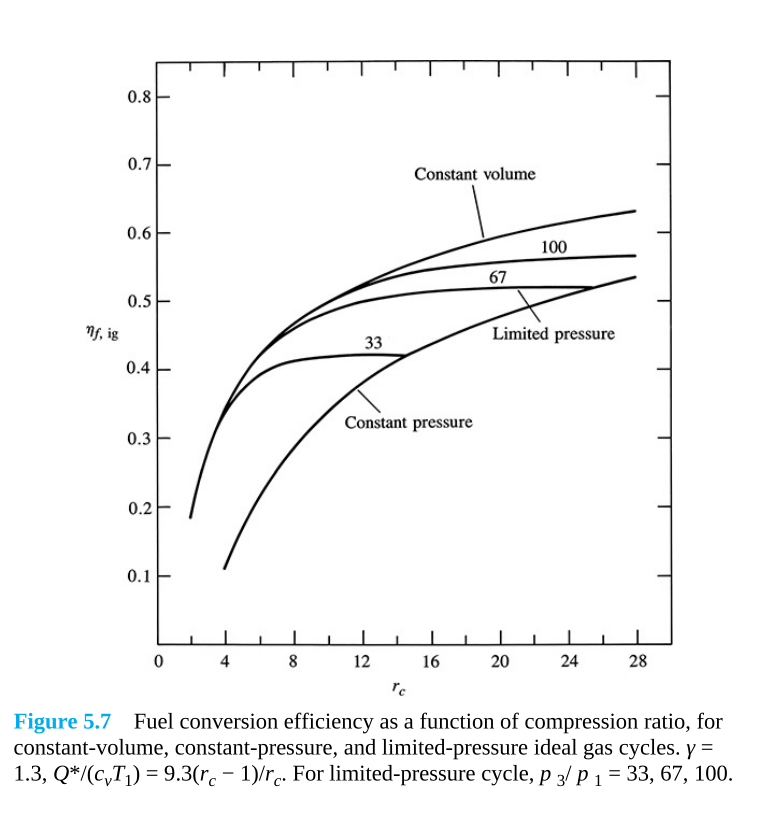
\includegraphics[width=.7\textwidth]{rendimiento_conv_comb.png}
    \caption{Rendimiento de conversión de combustible en función de $r_c$ para
ciclos de gas ideal de volumen constante, presión constante y presión
limitada} \label{fig:rendimientos}
    %
\end{figure}


\subsection{Propiedades termodinámicas de mezclas aire-combustible}\label{subsec:prop_mezcla}
%
Fue necesario estimar las propiedades termodinámicas de la mezcla para obtener
algunas variables utilizadas para calcular las condiciones iniciales del gas en
las flujometrías.
%
En lo que respecta a la simulación del ciclo del motor, ICESym contiene rutinas
computacionales para calcular el estado termodinámico del fluido de trabajo en
el ciclo operativo.
%
En este apartado se detallan las hipótesis y modelos utilizados en las rutinas
computacionales para el cálculo de las propiedades termodinámicas de las mezclas
de aire-combustible quemadas y sin quemar, para el uso en las condiciones
iniciales requeridas en las flujometrías.

En la simulación del MRCVC se utilizó una mezcla estequeométrica ($\phi=1$) de
aire-isooctano $C_{8}H_{18}$ cuya reacción (estequeométrica) se indica en la
ecuación \ref{eq:estequeometrica}.

\begin{equation} \label{eq:estequeometrica}
  C_{8}H_{18} + 12.5 \left(O_{2}+3.772N_{2}\right) \rightarrow 8 CO_{2} + 9 H_{2}O + 47.16 N_{2}
\end{equation}

Expresando el combustible de manera genérica con $C_{a}H_{b}$ o en función de la
cantidad de moles de carbono del combustible $CH_{y}$ con $y=\frac{b}{a}$, se
puede expresar la proporción estequeométrica de aire combustible que se
requiere con la ecuación~\ref{eq:rel_as}.

\begin{equation} \label{eq:rel_as}
  \left(\frac{A}{F}\right)_{s} = \left(\frac{F}{A}\right)_{s}^{-1} = \frac{34.56(4+y)}{12.011 + 1.008y}
\end{equation}


Otro número importante es la relación de equivalencia $\phi$, que se calcula con
el cociente entre la relación molar real y estequeométrica de una mezcla, ver
ecuación~\ref{eq:phi}

\begin{equation}\label{eq:phi}
  \phi = \frac{{(F/A)}_{real}}{{(F/A)}_{s}}
\end{equation}

Las rutinas computacionales utilizadas para calcular las propiedades
termodinámicas de las mezclas aire-combustible aproximan las mismas con curvas
polinómicas asumiendo que: 1) la composición de la mezcla sin quemar está,
congelada 2) la mezcla de gases quemados se encuentra en equilibrio químico.

La composición de la mezcla no cambia significativamente durante los procesos de
admisión y compresión, por lo que se asume que la mezcla está congelada.
%
Durante la combustión y parte del proceso de expansión se asume que la mezcla de
gases quemados está cerca del equilibrio termodinámico, a medida que los gases
se enfrían en durante la expansión, se puede asumir que la composición química
se congela.

Para cada compuesto $i$ de la mezcla a temperatura estándar $T(K)$ y 1 atmósfera
de presión se aproxima el calor especifico a presión constante
$\widetilde{c_{p,i}}$ por la ecuación~\ref{eq:cp}, la entalpía estándar
$\widetilde{h_{i}}$ por la ecuación~\ref{eq:h} y la entropía estándar
$\widetilde{s_{i}}$ por la ecuación~\ref{eq:s}.

\begin{equation}\label{eq:cp} \frac{\widetilde{c_{p,i}}}{T} = a_{i1} + a_{i2}T + a_{i3}T^{2} + a_{i4}T^{3} + a_{i5}T^{4}
\end{equation}

\begin{equation}\label{eq:h} \frac{\widetilde{h_{i}}}{\widetilde{R}T} = a_{i1} + \frac{a_{i2}}{2}T + \frac{a_{i3}}{3}T^{2} + \frac{a_{i4}}{4}T^{3} + \frac{a_{i5}}{5}T^{4} +\frac{a_{i6}}{T}
\end{equation}


\begin{equation}\label{eq:s} \frac{\widetilde{s_{i}}}{\widetilde{R}} = a_{i1} \ln{T} + a_{i2}T + \frac{a_{i3}}{2}T^{2} + \frac{a_{i4}}{3}T^{3} + \frac{a_{i5}}{4}T^{4} + a_{i6}
\end{equation}

La base de datos seleccionada para los datos del aire y productos de la
combustión es Chemkin~\parencite{chemkin} y los datos del isooctano de
Raine~\parencite{raine}.

La finalidad de estas rutinas (por fuera de las incuidas en ICESym) es la de
obtener la masa molar de la mezcla $M_{M}$, la viscosidad dinámica $\mu$, calor
específico a presión constante $C_{P}$, gamma $\gamma$ y el número de Prandtl
$P_{R}$, ya que todos estos valores son requeridos para obtener las condiciones
iniciales de las flujometrías.

La masa molar de la mezcla $M_{M}$ se calcula a partir de la suma de las masas
molares $M_{i}$ y la fracicón molar de cada especie química presente en la
mezcla $x_{i}$, ver ecuación~\ref{eq:mw}.
%
La viscosidad $\mu$ de los productos de la combustión de aire e hidrocarburos
para temperaturas de entre $T\in [500, 4000]K$, $P\in[1, 100]atm$ y
$\phi \in [0,4]$ se puede aproximar en función de la temperatura y la relación
de equivalencia con la ecuación~\ref{eq:mu}.
%
Del mismo modo, el número de Prantl de productos de la combustión de
hidrocarburos y aire se puede estimar en función del $\gamma$ de la mezcla, para
$\phi\leq 1$ con la  ecuación~\ref{eq:pr}

\begin{equation}\label{eq:mw}
  M_{m} = \sum_{i} M_{i}x_{i}
\end{equation}

\begin{equation}\label{eq:mu}
  \mu_{productos} = \frac{\mu_{aire}} {1 + 0.027 \phi} = \frac{3.3\times 10^{-7} T^{0.7}} {1 + 0.027 \phi}
\end{equation}

\begin{equation}\label{eq:pr}
    \Pr = 0.05 + 4.2 (\gamma - 1) - 6.7 {(\gamma - 1)}^{2}
\end{equation}
